\documentclass{report}
\usepackage{graphicx, chemformula, titlesec,pdfpages}
\usepackage[a4paper, portrait, margin=1in]{geometry}
\usepackage[table,xcdraw]{xcolor}
\title{Accreditation course in radiation protection - Radiation Protection Officer – Dispersible radioactive substances level D (TMS-VRS D)}
\date{September 2025}
\author{Mar Roca Cugat}
\begin{document}
\maketitle
\tableofcontents
%-------------------------------------------------------------------------------------------------------------------------------------------------------------------------------------------------------------------------------------------------------------------------------------------------------------------------------------%x
\part{Quick reference handbook}
\chapter{Radioactive decay}
\textbf{$\alpha$ decay}: Occurs when the nucleus is unstable, due to being too big. The parent atom $\ch{^{A}_{Z}X}$ gets split into a daughter atom $\ch{^{A-4}_{Z-2}Y}$ and an alpha particle $\ch{^{4}_{2}a}$.\\\\
\textbf{$\beta^{-}$ decay}: Occurs when the nucleus is unstable, due to having an excess of neutrons. The parent atom $\ch{^{A}_{Z}X}$ gets split into a daughter atom $\ch{^{A}_{Z+1}Y}$, a beta particle $\ch{^{0}_{-1}e^{-}}$, and an anti-neutrino $\overline{v}_e$.\\\\
\textbf{$\beta^{+}$ decay}: Occurs when the nucleus is unstable, due to having an excess of protons. The parent atom $\ch{^{A}_{Z}X}$ gets split into a daughter atom $\ch{^{A}_{Z+1}Y}$, a positron $\ch{^{0}_{+1}e^{+}}$, and a neutrino $v$. After a number of interactions, the positron $\beta{+}$ unites with an electron and converts its entire mass to energy. This annihilation produces 511 keV.\\\\
\textbf{Electron capture}: The nucleus absorbs an electron from the electron cloud (usually from shell K -innermost). The parent atom $\ch{^{A}_{Z}X}$ absorbs an electron $\ch{^{0}_{-1}e^{-}}$, and gets split into a daughter atom $\ch{^{A}_{Z-1}Y}$, and a neutrino $v$.\\\\
\textbf{Gamma decay ($\gamma$)} Occurs when the atom is excited. The parent atom $\ch{^{A}_{Z}X*}$ gets excited and produces a daughter particle $\ch{^{A}_{Z}X}$ and a gamma ray $\gamma^{1}$. Internal conversion may occur (direct transsfer of the energy of the nucleus to an electron).
%--------------------------------------------------------------------------------------------------------------------------------------------------------------------------------------------------------------------------------------------------------------------------------------------------------------------------%
\chapter{Formulas}
\section{Activity determination}
\[A(t) = A(0) \cdot (\frac{1}{2})^{\frac{t}{T_{1/2}}}\]
\textbf{Precise determination with a formula for the half-life using half-life}. All time units must be in the same unit.\\
\[\frac{dN(t)}{dt}=-\lambda\cdot N(t);\ A(t) = A(0)\cdot e^{-\lambda t}\]
\textbf{Precise determination with a formula for the half-life using decay constant ($\lambda$)}. All time units must be in the same unit.\\

\section{Shielding}
\[g \approx 2\cdot10^{-4}\cdot Z\cdot E_{\beta,max}\]
\textbf{Approximation of the energy converted to Bremsstrahlung}. Where $Z$ is the atomic number of the shielding material\\
\[R_{\beta,\ in\ material} = \frac{R_{\beta,\ in\ water} = 0.5 E_{\beta,max}}{\rho_{material}}\]
\textbf{Range of $\beta$ particle in a specific material}. For water and tissue, $\rho$ can be estimated to be 1 g/cm³. $E_{\beta,max}$ is expressed in MeV.\\
\[I(d) = I(0)\cdot B\cdot(\frac{1}{2})^{\frac{d}{d_{1/2}}}\]
\textbf{Shielding of $\gamma$ radiation using half distance}. Buildup factor (P60) may be ignored. All distance units must be in the same unit.\\
\[I(d) = I(0)\cdot e^{-\mu_{linear} d}; \mu_{mass} = \mu_{linear}\cdot\rho_{material}^{-1}\]
\textbf{Shielding of $\gamma$ radiation using linear attenuation coefficient}. Above 500keV, $\mu_{mass\ water}\approx\mu_{mass\ concrete}$.\\

\section{Dose determination}
\[H_T = W_R \cdot D\]
\textbf{Equivalent dose}. $W_R$ is the radiation weighting factor: 1x for $\beta$ and $\gamma$, 20x for $\alpha$, and 2-20x for $N_0$. D is the absorbed dose over tissue of organ (Gy).\\
\[E = \sum (W_T \cdot H_T)\]
\textbf{Effective dose}. $W_T$ is the tissue weighting factor (P64). \\
\[E(50) = e(50)\cdot A\]
\textbf{Committed effective dose (Sv)}. e(50) is the committed effective dose coefficient (Sv$\cdot$Bq$^{-1}$).\\
\[\cdot H*(10) = h(10)\cdot\frac{A}{r²}\]
\textbf{Inverse square law}. The activity must be in MBq, the distance in m, and the result in $\mu$Sv/h\\
\[X\]
\textbf{}\\

\section{Measurement}
\[rel. error = \frac{\sqrt{N}}{N} = \frac{1}{\sqrt{N}}\]
\textbf{Relative error}. $N$ is the number of counted pulses, $\sqrt{N} is the counting error$\\
\[\epsilon = \frac{R}{A}\]
\textbf{Efficiency}, where R is the counting rate in units of per second, and A is the activity in Bq.\\
%--------------------------------------------------------------------------------------------------------------------------------------------------------------------------------------------------------------------------------------------------------------------------------------------------------------------------%
\chapter{Useful information}
\begin{figure}
    \centering
    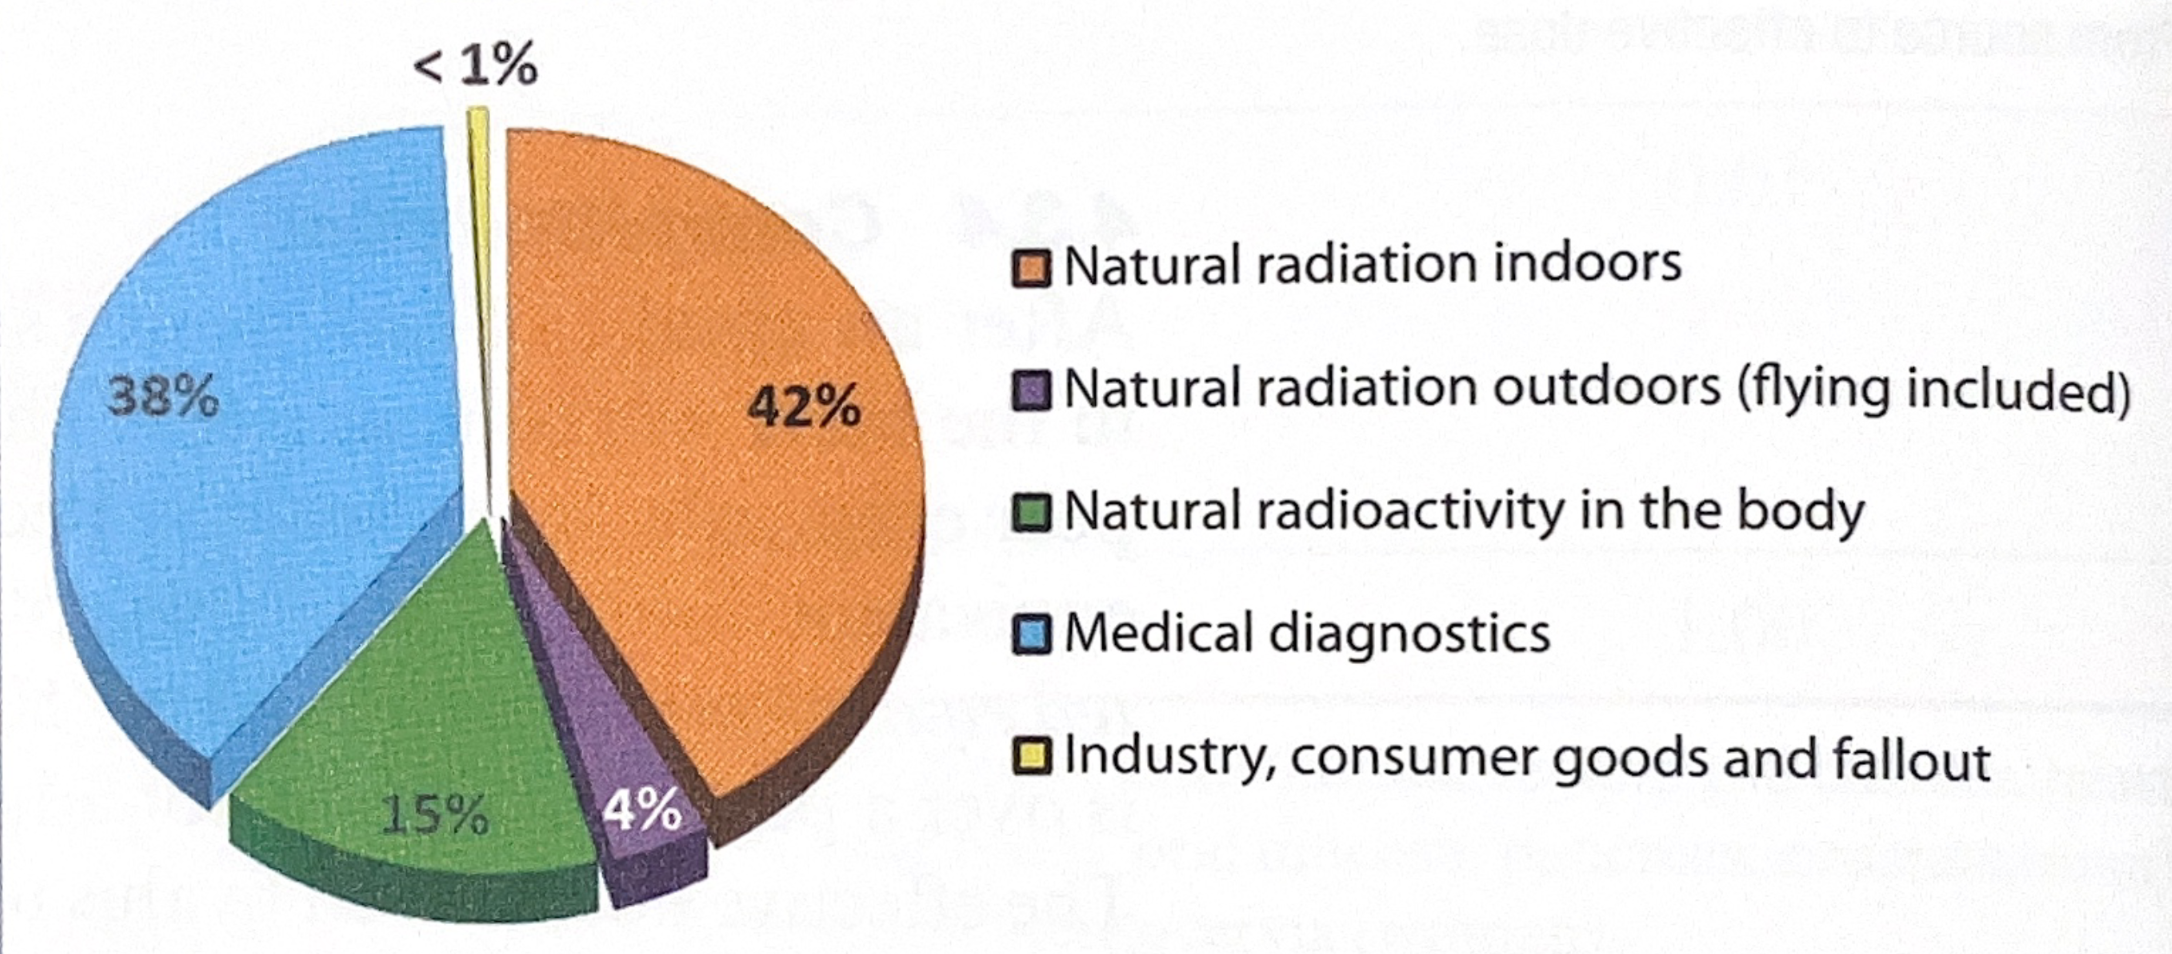
\includegraphics[width=0.5\linewidth]{Normal_dose.png}
    \caption{Contributions to the dose for a member of the public in the Netherlands}
    \label{fig:placeholder}
\end{figure}
\begin{table}[ht]
\caption{Detectors and their usual applications}
\label{detect}
\begin{tabular}{lll}
\hline
 & $\beta$ emitters & Photon radiation \\ \hline
\textbf{Ionisation detectors} &  &  \\
GM Tube (thin window) & Contamination & Contamination \\
GM Tube (thick window) & - & Dose rate \\
Proportional counter (thin window, xenon filled) & Large area contamination & Large area contamination \\for low-energy photons \\
Germanium semiconductor & - & Accurate spectrum \\ \hline
\textbf{Scintillation detectors} &  &  \\
Nal(Tl) & - & \begin{tabular}[c]{@{}l@{}}Contamination\\ Simple spectrum\\ Dose rate\end{tabular} \\
Andthracene or ZnS & Contamination & Contamination \\
TLD & Personal dosimeter & Personal dosimeter \\
 &  & 
\end{tabular}
\end{table}
%----------------------------------%
\begin{table}[ht]
\caption{Dose limits}
\label{doses}
\begin{tabular}{llll}
\rowcolor[HTML]{343434} 
\multicolumn{1}{l|}{\cellcolor[HTML]{343434}{\color[HTML]{FFFFFF} \textbf{Group}}} & \multicolumn{1}{l|}{\cellcolor[HTML]{343434}{\color[HTML]{FFFFFF} \textbf{\begin{tabular}[c]{@{}l@{}}Effective dose [mSv/y]\end{tabular}}}} & \multicolumn{2}{l}{\cellcolor[HTML]{343434}{\color[HTML]{FFFFFF} \textbf{\begin{tabular}[c]{@{}l@{}}Equivalent dose [mSv/y]\end{tabular}}}} \\
\rowcolor[HTML]{C0C0C0} & \multicolumn{1}{l|}{\cellcolor[HTML]{C0C0C0}{\color[HTML]{333333} Total body}} & \multicolumn{1}{l|}{\cellcolor[HTML]{C0C0C0}{\color[HTML]{333333} Eye lens}} & {\color[HTML]{333333} Skin \& extremities} \\ \hline
\textbf{Category A} & 20 & 20 & 500 \\
\textbf{\begin{tabular}[c]{@{}l@{}}Category B\\ Exposed pupils and students\\ Those between 16 and 18\end{tabular}} & 6 & 15 & 150 \\
\textbf{\begin{tabular}[c]{@{}l@{}}Category C\\ ``Non-exposed employees''\end{tabular}} & 1 & 15 & 50 \\
\textbf{Pregnant employees} & \multicolumn{3}{l}{Maximum 1 mSv equiv to abdomen from announcement to birth.} \\
\textbf{\begin{tabular}[c]{@{}l@{}}Members of the public\\ Excluding patients\end{tabular}} & 1 & 15 & 50
\end{tabular}
\end{table}































%\[X\]
%\textbf{}\\
%-------------------------------------------------------------------------------------------------------------------------------------------------------------------------------------------------------------------------------------------------------------------------------------------------------------------------------------%
\setcounter{page}{1}\part{Classes}
\chapter{Physics 1}%-------------------------------------------------------------------------------------------------------------------------------------------------------------------------------------------------------------------------------------------------------------------------------------------------------------------------------------%
\section{Structure of an atom}
An atom of X element has Z number of protons, N number of neutrons [n(0)], and a mass (A) of Z+N. \\
An element can be expressed as $\ch{^{A}_{Z}X}$ \par.
%-------------------------------------------------------------------------------------------------------------------------------------------------------------------------------------------------------------------------------------------------------------------------------------------------------------------------------------%
\section{Radioactive decay}
Decay may occur due to:
 \begin{enumerate}
	\item Too many protons
	\item Too many neutrons
	\item Too many neutrons and protons
	\item Energetically excited state
\end{enumerate}
The chart of nucleides expresses in black the stable nuclei and in white the unstable nuclei. Isobars have the same mass (A), and isotopes have the same number of P+ (Z).
%-------------------------------------------------------------------------------------------------------------------------------------------------------------------------------------------------------------------------------------------------------------------------------------------------------------------------------------%
\section{Ionizing radiation}
Radiation is energy released as electromagnetic waves or particles. \\
Ionisation means removing electrons from the electron cloud of the atom. \\
Ionising radiation can consist of:
 \begin{enumerate}
	\item Particle radiation (with high energy)
	 \begin{enumerate}
		\item Alpha decay
		\item Beta decay
		\item Electron capture
		\item Positron emission
	\end{enumerate}
	 \item Electromagnetic radiation (with high energy)
	 \begin{enumerate}
		\item Isomeric transition (gamma emission)
	\end{enumerate}	 
\end{enumerate}
The radiation type that occurs can be seen on the chart of nucleides (see slide 10). 
\subsubsection{Alpha decay ($\alpha$)}
Occurs when the nucleus is unstable, due to being too big.\\
The parent atom $\ch{^{A}_{Z}X}$ gets split into a daughter atom $\ch{^{A-4}_{Z-2}Y}$ and an alpha particle $\ch{^{4}_{2}a}$.
\subsubsection{Beta decay ($\beta$)}
Occurs when the nucleus is unstable, due to having an excess of n.\\
The parent atom $\ch{^{A}_{Z}X}$ gets split into a daughter atom $\ch{^{A}_{Z+1}Y}$, a beta particle $\ch{^{0}_{-1}e^{-}}$, and an anti-neutrino $\overline{v}_e$.
\subsubsection{Electron capture (E.C. or $\epsilon$)}
Occurs when the nucleus is unstable, due to having an excess of p.\\
The parent atom $\ch{^{A}_{Z}X}$ absorbs an electron $\ch{^{0}_{-1}e^{-}}$, and gets split into a daughter atom $\ch{^{A}_{Z-1}Y}$, and a neutrino $v$.
If the hole is filled by an outer shell electron, X-rays are emmitted.
[...]
\subsubsection{Positron emission ($\beta^{+})$}
Occurs when the nucleus is unstable, due to having an excess of p.\\
The parent atom $\ch{^{A}_{Z}X}$ gets split into a daughter atom $\ch{^{A}_{Z+1}Y}$, a positron $\ch{^{0}_{+1}e^{+}}$, and a neutrino $v$.
After a number of interactions, the positron unites with an electron and converts its entire mass to energy. This annihilation produces 511 keV.
\subsubsection{Gamma decay ($\gamma$)}
Occurs when the atom is excited.\\
The parent atom $\ch{^{A}_{Z}X*}$ gets excited and produces a daughter particle $\ch{^{A}_{Z}X}$ and a gamma ray $\gamma^{1}$.
%-------------------------------------------------------------------------------------------------------------------------------------------------------------------------------------------------------------------------------------------------------------------------------------------------------------------------------------%
\section{Activity}
\subsection{Unit of activity (A)}
The unit of activity is the Becquerel (Bq). 1 Bq = 1 disintegration per second.
The specific activity is the activity per mass (Bq/g)
The old unit was Curie (Ci), equivalent to $3.7·10^{10}Bq$
 \subsection{Decay law}
 Decay is a random process. 
Activity is proportional to the number of nuclei and the decay constant $\lambda (s^{-1})$:
\[ A = -\frac{dN}{dt} = \lambda N \]
The half life is the number of seconds that it takes to decay half of all nuclei present:
\[ t_{1/2} = -\frac{ln2}{\lambda} = \frac{0.693}{\lambda} \]
The activity ($A_t$) on time (t) can be approximated as:
\[ A_{t} = A_0 * e^{-\frac{t}{t_{1/2}}*ln(2)} \]
\[ A_{t} = A_0 * \frac{1}{2}^{-\frac{t}{t_{1/2}}} \]
%-------------------------------------------------------------------------------------------------------------------------------------------------------------------------------------------------------------------------------------------------------------------------------------------------------------------------------------%
\section{Electromagnetic radiation}
Electromagnetic radiation is non-material. \\
The smaller the wavelength, the higher the frequency, and the higher the energy.
\[ \lambda = \frac{c}{v} \]
\[E = \frac{hc}{\lambda} = h*v \]

\subsection{Generation of X-rays}
X-rays happen when high energy atoms are slowed down by matter. An atom is bombarded by electrons. When an electron hits another electron, a hole is formed. This is then filled by an electron from the electron shell, which releases energy. Three situations can occur: 
 \begin{enumerate}
	\item The electron can hit the nucleus, which produces the maximum energy.
	\item The electron can have a close interaction, which produces moderate energy.
	\item The electron can have a distant interaction, which prouces low energy.
\end{enumerate}
The X-ray tube produces X-rays. It depends on the electron energy (regulated by the tube voltage), and the anode material (usually tungsten). <1\% of energy is converted to X-rays, and the rest is heat. 
The X-ray tube has a spectrum of emission, called the Spectrum Bremsstrahlung.
In an X-ray spectrum there's always peaks. Those are called the characteristic X-rays, and they depend on the material. X-rays can be filtered or unfiltered. This reduces the amount of X-rays in the areas that aren't of interest. The filter affects the X-rays differently depending on the material it's made out of.

\subsection{Interaction of radiation with matter}
Gamma and X-rays can interact with matter in the following ways:
 \begin{enumerate}
	\item Classic scattering (mainly non-ionising radiation)
	\item Photo effect
	\item Compton effect
	\item Pair production
\end{enumerate}
Which method occurs depends on the photon energy and the atomic number (see slide 61)
\subsubsection{Classic scattering}
Also called elastic, coherent or Rayleigh scattering.
Gamma energy remains unchanged, but the direction of the photon may change. It is important at low $E_{\lambda}$

\subsubsection{Photo effect}
The photon knocks an electron out of its orbit. The electron has binding energy, so the resulting energy is minimal. It goes up to 0.5MeV. The chance is roughly proportional to $Z^4$, and it produces characteristic X-rays.

\subsubsection{Compton effect}
The dominant effect at higher energies. Depends on the material.
The photon is scattered at weakly bound electrons, transferring partly the energy to the electron. However, it continues and may hit another electron. It can go through the material, with less energy that it came in.
The degree of energy transfer depends on the scatter angle. The maximal energy will be at 180ª, and the minimal energy at 0º. With a portable X-ray tube it's better to have it below the bed, as it's shielded, and most of the backscatter will go to the rear.

\subsubsection{Pair production}
Near the nucleus, the photon can create both an electron and a positron, if it has enough energy. This usually results in an annihilation, usually outside of the atom, creating 2 511keV photons, at 180º from each other. This can only occur at energies of over 1.022MeV (mass of the electron + positron). 


\chapter{Physics 2}%-------------------------------------------------------------------------------------------------------------------------------------------------------------------------------------------------------------------------------------------------------------------------------------------------------------------------------------%
\section{Interaction of charged particles with matter}
Photons do not experience energy loss per distance. However, charged particles do. There is a certain amount of energy loss per cm (LET: Linear Energy Transfer), or Stopping Power. Alpha particles have a high stopping power, as they lose a lot of energy at a short distance.\\
The range is the maximum distance that charged particles can travel in matter. It depends on the type of charged particle, the energy of the charged particle, and the density of the material. Not every electron has the same speed, as the energy is distributed unequally and randomly between the electron and the neutrino. The mean energy is lower than the 50\% of the range. \\
Rule of thumb (produces an overestimation) for $\beta$ with E > 0.6 MeV:
\[ R (cm) * \rho (\frac{g}{cm³} )= 0.5\ E_{\beta,max} (MeV) \]
Soft tissue is very equivalent to water, and thus can be approximated to a density of 1. Air is around 1000 times higher.

\subsection{Interaction of $\alpha$ particles with matter}
Due to the interaction with the electrons of atoms (ionizations and excitations), the energy of an $\alpha$ particle decreases. It disposes of its energy linearly along a straight path. The range/pathway depends on the energy of the radiation and the density of the material\\
Alpha particles have a high stopping power. They lose a lot of energy at a short distance (small range, thick track). They are unable to pass the epidermis, but they are very dangerous if ingested. \\

\subsection{Interaction of protons with matter}
Protons behave like $\alpha$ particles, but they can be directed to deposit most of their energy at a specific point (Bragg peak). The Bragg peak can be manipulated with the energy.

\subsection{}


\subsection{Shielding from ionizing radiation}
Shielding for particles only needs to be as thick as the maximal range. However, for photons, you the shielding needs to be as thick as deemed reasonably safe. \\
The $\gamma$-photon pathway is much longer than the $\beta$-particle, which is longer than the $\alpha$-particle pathway.
\subsubsection{Alpha}
For $\alpha$ particles, barely any shielding is necessary. 
\subsubsection{Beta}
For $\beta$ particles, the rule of thumb can be applied. Shielding materials with a low Z-value cause less Bremsstrahlung. Such materials are Perspex or aluminum (mostly Perspex, as it's see-through, and has an even lower Z-value). Bremsstrahlung causes a loss of energy, which is released as a photon, usually in the X-ray range. $\beta$ emmitters are usually stored in a perspex container in a lead container. Perspex is often used a a mimic for tissue.
\subsubsection{Gamma}
For $\gamma$ and X-rays, the material cannot stop them entirely but rather attenuate them. It depends on the energy of the radiation, and the density of the material (or rather Z value, the highest Z-value attenuates the most). The attenuation can be calculated with:
\[  I_d = I_0\ e^{-\mu d}   \]
Where d is the thickness of the material and $\mu$ is the attenuation coefficient. After $d_{1/2}$, the photon intensity is halved:
\[  d_{1/2} = \frac{ln2}{\mu}  \]
Transmission is the ratio between the original intensity and the dampened intensity.
\[  T = \frac{I_d}{I_0}	 \]

\subsection{Inverse square law}
Electromagnetic radiation is a Newtonian form of radiation, which means that it decreases in intensity by the square of the distance. This is because the intensity is the number of photons/sm², and the surface of a sphere increases with the square of the radius.

\section{Dose}
\subsection{Definition of dose}
An absorbed dose (D) is the absorbed energy per mass of matter. We use the Gray (Gy), equivalent to 1 Joule/kg.
\subsection{Calculation of a $\gamma$ dose rate}
\[ H = \frac{h(10)A}{r^2} \]
Where h(10) is the ambience dose equivalent rate/source constant, H is the dose rate, A is the activity, and r is the distance.\\
The h(10) is exclusive for nucleides with gamma emission. There's tables that can be used.
\subsection{Rules of thumb}

\subsubsection{$\beta$ radiation}
The source of an A MBq source that emits a $\beta$ particle of E MeV per decay event at 10 cm is
\[ H_{skin} = 1000A (\frac{\mu Sv}{h} \]

\subsubsection{$\gamma$ radiation}
The source of an A MBq source that emits a $\gamma$ photon of E MeV per decay event at 30 cm is
\[ H = 2A (\frac{\mu Sv}{h} \]

\subsection{Dose reduction}
 \begin{enumerate}
	\item Time $\rightarrow$ Work fast
	\item Distance $\rightarrow$ Stay away
	\item Shielding $\rightarrow$ Use shielding
	\item Activity $\rightarrow$ Use the minimum needed
\end{enumerate}

\subsection{Buildup factor}
The attenuation law assumes a narrow beam. However, that's not correct. Depending on the shielding material, there may be a lot of backscatter, which amplifies the radiation after the shielding. The build-up factor depends on the energy and the material, and it may need additional shielding to compensate. The buildup factor can be considerable, commonly factor 2-4, but even goes higher than 100.

\subsection{Dose and biology}
\begin{table}[]
\begin{tabular}{llll}
Quantity        & Symbol & Unit         & Type       \\
Absorbed dose   & D      & Gray (Gy)    & Physical   \\
Equivalent dose & $H_T$    & Sievert (Sv) & Biological (Specific part) \\
Effective dose  & E      & Sievert (Sv) & Biological (Whole body)
\end{tabular}
\end{table}

\subsubsection{Equivalent dose}
The seriousness of biological tissue damage is also determined by the way that energy is disposed. It depends on the kind of radiation. $\alpha$ radiation has more ionizations per path length, so it does more damage than $\beta$ or $\gamma$.
\[ H_T = D * W_R\]
Where $W_R$ is the radiation weighting factor, and D is the absorbed dose in Gray

\begin{table}[]
\begin{tabular}{ll}
Type of radiation & $W_R$    \\
$\beta$             & 1      \\
$\gamma$            & 1      \\
X-ray             & 1      \\
n                 & 5-20   \\
p                 & 1.1-10 \\
$\alpha$            & 20    
\end{tabular}
\end{table}

\subsubsection{Effective dose}
It is a quantity used for comparison of risks. The effective dose is the radiation dose needed in homogenous total body irradiation to obtain the same risk.
\[ \sum_{T}^{}H_T\cdot W_T \]
Where $H_T$ is the equivalent dose and $W_T$ is the tissue weighting factor (See Table 5.2 in the book). $W_T$ depends on the rate of division of the cells in each organ.

\subsubsection{Dose Conversion Coefficients}
To calculate the effective (committed = internal) dose after contamination (ingestion) with radionucleides, the following formula is used:
\[ E_{committed} = A*e_{50}\]
E(50) is the effective dose received over 50 years after intake, and it depends on the chemical form, way of intake, and sometimes disease of the patient. The e(50) or DCC or $e_{inh/ing}$ is a coefficient that can be looked up on tables.

To calculate the effective dose after skin contamination, e(50) (Sv/Bq) and $DCC_{skin}$ (mSv/s per kBq/cm²) are used for contamination, h(10) is used for irradiation ($\mu$ Sv/h per MBq/m²)

\chapter{Measuring methods}The purpose of measuring is to determine the type of radiation, the activity, the energy of the radiation, or the (effective) dose or dose rate.
\section{Principles of radiation detection}
\begin{table}[]
\begin{tabular}{lll}
Principle of operation & Detector material                                                        & Detector type                                                              \\
Electrical charge      & \begin{tabular}[c]{@{}l@{}}Gas\\ Solid state\end{tabular}                & \begin{tabular}[c]{@{}l@{}}Gas-filled\\ Semiconductor\end{tabular}         \\
Luminescence           & \begin{tabular}[c]{@{}l@{}}Solid/liquid state\\ Solid state\end{tabular} & \begin{tabular}[c]{@{}l@{}}Scintillation\\ Thermoluminescence\end{tabular} \\
Chemical reaction      & Photographic emulsion                                                    & Densitometer                                                               \\
Warmth                 & Solid/liquid state                                                       & Calorimeter                                                                \\
Activation             & Solid state                                                              & Activation dose meter                                                     
\end{tabular}
\end{table}

\section{Ionization/Electric charge}
\subsection{Gas-filled detectors}
Gas-filled detectors have a closed tube that contain air or another gas. When radiation enters the tube, ionization occurs. The walls of the detector have a voltage between them, which separates the ions, and this can be measured through the current. The current is proportional to the primary electron-ion pairs, which is proportional to the absorbed amount of energy. However, these detectors have a a recombination region (Applied voltage < Saturation voltage), in which they can work. Above the saturation voltage, there's the saturation region, in which the detector can't detect more because all formed ion pairs can reach the electrodes, and cannot recombinate. They consist of a tube with very thin membranes at the end (protected by a mesh or bars).\\

\subsubsection{Ionization chamber}
They produce very small electrical signals. They aren't used in pulse mode to detect indiviual counts, but rather used for radiation intensity. They are most suited to detect radiation with high energy deposition ($\alpha$ or $\beta$), or with high energy, but it's not efficient for $\gamma$ rays. It can be used as a dose calibrator to determine the amount of radioactivity of a known radioisotope.

\subsubsection{Proportional counter region}
At sufficiently high voltage, the accelerated primary electrons have enough energy to cause ionization themselves and form secondary electron pairs (cascade).\\
The proportional counter uses the proportional counter region. It produces larger electrical signals than the ionization chamber, so it is used in pulse mode to detect individual counts. The electrical signal is proportional to the amount of deposited energy, so it can be used for energy selective counting. It's most suited to detect radiation with high energy deposition ($\alpha$ and $\beta$), and though it can detect $\gamma$, it's not as efficient. It can be used as a contamination monitor.

\subsubsection{Geiger-Müller region}
Similar to the proportional counter region, but even more. This is called the avalanche. At high voltage, emission photons are created, which can interact with gas, creating even more electron-ion pairs. The avalanche is stopped when a large number of 'slow' positive ions reduces the effective voltage, and the electrical charge becomes independent of absorbed energy.\\
The Geiger-Müller counter uses the Geiger-Müller region. It produces larger electrical signals that can be easily measured with low cost electronics, so they are used in pulse mode. The electrical signal is independent of absorbed energy, so it's not used for energy-selective counting. It's inefficient for $\gamma$ rays, but it's more sensitive than the ionization chamber and the proportional counters. They are used as survey monitors.

\subsection{Semiconductors}
They work in a similar way to the gas-filled detectors, but they're more efficient for X- and $\gamma$-rays, given their higher stopping power. The energy needed to create a single electron-ion pair is much lower than for air, so a larger electrical signal is produced.\\
Individual counts can be measured with a very high energy resolution, which produces an energy spectrum, which is a 'fingerprint' that is used to identify radio-isotopes.\\
In order to suppress noise they must be cooled, so they are immovile and very heavy.

\section{Luminescence}
\subsection{Scintillation}
They work through scintillations. This means that a photon is released in the UV or visible-light range when an excited electron returns to its ground state. The produced amount of light is proportional to the amount of energy. But this energy can be very small, so a photomultiplier tube is used by converting scintillation light to pulses of electrical current. The most common cathode is sodium iodide, or not as commonly, another salt. Radiation enters the crystal, and photons are released as a result.\\
Solid materials can be used, such as NaI or CsI (for $\gamma$ radiation), or anthracene or stilbene (plastics, used for $\alpha$ and $\beta$ radiation). Organic liquid materials can also be used to detect $\alpha$ or $\beta$ radiation (a small amount of sample is put in the liquid), and it's best used for low-energy sources, as it's often the only way to check for contamination (with swipe or smear tests).\\
Scintillation can also be used to identify materiials, although they have a lower resolution than semiconductors.

\subsection{Thermoluminescence}
It is often used in personal dosimeters. The thermoluminescent detector is made from a material that can emit photons upon heating after exposure to ionizing radiation. Therefore, it 'captures' radiation, and releases it when it's heated.

\section{Efficiency}
No detector is 100\% efficient. This is because even if the detector was perfect, you'd only be measuring by one side. The measurement efficiency depends on detector efficiency, geometric efficiency, the source, and the absorption between the source and the detector. The efficiency can be determined by measuring a source with known activity.
\[ \epsilon = \frac{R_{net}}{A} = \frac{R_{gross}-R_{background}}{A}\]
Where R<A, R being the count rate, and A being the actual activity. 

\section{Counting statistics}


\chapter{Biological Effects}\section{Effects of radiation on cells}
Everything in the cell is a possible target. However, the biggest risk is the nucleus, and its DNA. This is because it can create DNA damage, such as base damage, cross-links, single/double strand breaks. In oncology, double strand breaks are needed to treat cancer. 1Gy of LET X-rays produces 1000 single-strand breaks, 40 double-strand breaks and 1000 altered bases.

\subsection{DNA repair}
Cells have a lot of repair mechanisms. Double-stranded breaks can cause many errors due to non-homologous end-joining. NHEJ cuts corners for the sake of speed. Single-strand breaks are easily repaired, in a couple of minutes after irradiation, 80\% of breaks are repaired. Double-strand breaks take much longer, taking hours for the same 80\% of breaks being repaired. 

\subsection{Stochastic effects}
Chance is proportionally related to the dose. There's no threshold, any exposure is any damage. It can cause cancer or congenital defects. There may be a latency period. This is based on the multiple hit theory (multiple 'hits' are needed to cause cancer). The multiple hit theory says that multiple genetic changes are necessary. Oncogenes (such as Ras) are needed to quickly proliferate cells. Tumour supressor genes (such as p53 or RB1) are needed to prevent mutated cells from dividing. DNA-repair genes (such as HNPCC or BRCA) are needed to to repair the DNA. Leukemia is a more immediate form of cancer (around 10-20 years), but most other forms of cancer take at least 15 years. \\
However, electromagnetic radiation usually only makes around 5-7\% of the carcinogenic factors. This also includes the sun's radiation, radon gas from working inside (radon is formed in the same rocks that are used to make buildings). Cancer is a multi-factorial risk, so it's difficult to tell the cause of the cancer. However, risks can be estimated by having large groups of exposed and non-exposed individuals, knowing the exact dose everyone received, and having a big difference with background radiation. One example of research was the one done after Hiroshima and Nagasaki. They had over 85k subjects in the cohort, and it has been running since the atomic bombs. The subjects get questionnaires, medical checkups, etc. yearly. Using the position where everyone was in the city when the bombs hit, the dose was estimated, which ranged from 0.01 to 6 Gy. By this life span study, they found that stomach cancer had an excess risk. There was also an increased chance of lung cancer, due to inhaling fallout. In general, per whole-body 1Gy dose, cancer risk increased by 47\%.  For those who received over 2 Gy, 56\% of cancers were caused by that dose. The age also increases the effect of the cancer. The younger at which you're exposed, the higher the chance of cancer. \\
The risk of malignancy was set to 5\%/Sv for 'civilians', and for workers 4\%/Sv. This is because in 'civilians' it's usually because of accidents, with a high dose at once; while in workers it's a lower dose spread through many years, which is more repairable. \\
Cancer is not the only type of stochastic effect. There's also genetic effects, which are hereditary. This damage is induced before conception, and may skip several generations. It is therefore difficult to study these effects in humans, so we only have animal studies. The studies also only use high doses (>0.5 Gy). A linear dose-effect relation without threshold is assumed. Only the damage in live births is accounted for. One such research was the MegaMouse project (>7000 mice). They looked at 6 types of hair colour and stunted ears. They found that not all the mice were equally sensitive, that repair time before procreation decreased the mutation frequency, and that there was a dose rate effect (high dose rate causes more damage than a low dose rate). From those experiments, there was a risk number of 1\%/Sv and a high spontaneous incidence of 10-20\% of genetic effects. The individual genetic effects are low. \\
Radiation during pregnancy is quite risky. The later the fetus is, the lower the risk to it is. During the preimplantation period (0-10 d), cells are pluripotent, so they can replace each other. Any damage results in apoptosis. It's an all-or-nothing effect, if the fetus survives, the child will not have effects. If not, the period will occur normally. During the organogenesis period (3-8 w), congenital malformations may occur. The effects are deterministic, with a threshold dose of 100 mSv. During the fetal period (8-25w) there's a growth delay, which may cause mantal retardation with a threshold dose of 100mSv, and after that a 10-40\% chance per Sv, with about 30 IQ points loss per Sv. The childhood malignancy is at 6\%/Sv. There's an increased risk of adult malignancy in life (2-3x). The fetal sensitivity is highest during the 1st trimester. With a dose below 100 mSv, the stochastic effects are unlikely, and there's no harmful tissue reactions. A dose above 500 mSv justifies abortion, as the risks are too high. The law sets an absolute limit from notification until birth of 1 mSv.

\subsection{Deterministic effects}
Deterministic/harmful tissue reactions depend on the dose. It takes a certain dose (threshold dose) to see effects in a certain amount of people (5\% of people see the effect). Below the threshold dose, the effects are unlikely. However, the sensitivity depends on the person, based on how fast their cells repair DNA. It seems like this resistance does not always transmit to the cancer.\\
With stochastic effects, even with a very low dose, there is a possibility of cancer, even if very small. It is a very cautious approach. That's why the dose given to the general population should be as low as reasonably achievable. The higher the cumulative lifetime dose, the higher the chance of getting effects (cancer or hereditary effects). However, it is a binary effect: you get cancer or you don't, regardless of dose.\\
DNA damage can cause cell death (resulting in the loss of organ function or sterility - harmful tissue reactions/deterministic effects), mutations (resulting in cancer or hereditary defects - stochastic effects), or repair. \\
Acute harmful tissue reactions can be seen immediately or delayed. Immediate reactions  are mainly cell loss, followed by an inflammatory response. Cell loss can result in anaemia, neutropenia, thrombopenia, epidermolysis, hair loss, ulceration... The following inflammatory response can result in mucositis, cystitis, enteritis, encephalitis, erythema, periostitis, keratitis... Late harmful tissue reactions can include atrophy, damage to blood vessels, chronic inflammatory reactions, fibrosis, sclerosis, necrosis... The effects vary by organ, as they have different sensitivities.\\
One famous case of carelessness is that of two interventional radiologists, and two nurses in 2 hospitals in Spain. They all developed cataract in both eyes, within two years. They were completely unknowledgeable about radiation protection. They didn't wear enough protection. There was no overhead shielding. They reached 0.45-0.9 Sv/y for several years.\\

\subsection{Dose limits}
In normal work, no harmful tissue reaction will be seen. There's dose limits which are set well below the damage threshold. The responsability of protection falls on the institution, not the worker. For 'civilians', the limit is 1 mSv/y. For radiation workers, the limit is 20 mSv/y. The damage is first seen at 2000 mSv.\\
%-------------------------------------------------------------------------------------------------------------------------------------------------------------------------------------------------------------------------------------------------------------------------------------------------------------------------------------%
\chapter{Risks and Risk Perception}\section{Ways of radiation exposure}
Average yearly dose per person in the Netherlands
\begin{enumerate}
	\item Medical applications (1-1.2 mSv) - Medical diagnostics (X-ray, CT, PET, SPECT)
	\item Radon in housing (0.64-1.37 mSv)
	\item Food (0.43 mSv) - Vegetables, meat and fruit have $\ch{^{40}_{}K}$, $\ch{^{210}_{}Pb}$, and $\ch{^{210}_{}Po}$. Fish have $\ch{^{137}_{}Cs}$
	\item Building materials (0.34 mSv) - Concrete and sheet rock have $\ch{^{226}_{}Ra}$, $\ch{^{232}_{}Th}$, and $\ch{^{40}_{}K}$.
	\item Cosmic radiation (0.22 mSv) - Mostly charged particles ($P^+$ and $e^-$)
	\item Terrestial radiation (0.03 mSv) - Depends on the soil type (Granite has $\ch{^{238}_{}U}$)
	\item Air traffic (increased cosmic radiation) (0.04 mSv)
	\item Radiation from atomic bombings (<0.01 mSv)
\end{enumerate}
Total 2.8 mSv per year. Zuid-Limburg has a lot more background radiation than most of the Netherlands, due to higher amount of radon in residential houses. Mountain ranges tend to have higher background radiation. However, as far as science knows, radiation does not seem to have an effect in life expectancy. \\
Belgium has a higher amount of Radon because it's on top of a lot of granite deposits. In Belgium they also do a lot more CT than the rest of the world. In the US, if you can afford it, they give you a lot of CTs.\\

\section{Risks and effects of ionizing radiation}
Ionizing radiation is harmful for the exposed individual, as well as for the individual's offspring. It causes short and long-term effects. We know it's dangerous because of history (Radium girls, Radithor, X-ray shoe fittings, radioactive toothpaste...). However it does have a few benefits, from medical diagnostics to safety. 
\subsection{Effects}
After Hiroshima and Nagasaki, Leukemia peaked around 10 years later, and all-type cancer around 35 years later. There's a dose-effect relation. We work with low amounts of radiation, through a long time of exposure. The Life Span study has drawbacks: it was a high dose rate at a short time of exposure, it was a total body exposure, and it was a specific type of exposure. This makes it difficult to use to calculate risks associated to work. Per Sievert of total body exposure, there's a 4-5\% of developing a fatal cancer. Per Sievert of exposure to the gonads, there's a 1\% chance at developing severe genetic damage in the offspring.\\
Hormesis is the beneficial effects due to low levels of radiation (homeopathic). There's no scientific proof (yet). The accepted model is the linear-no threshold model (any radiation is harmful).\\

\section{Risk perception}
Public perception is quite negative, and it is mostly affected by a few accidents. Radiophobia is an unfounded perceived risk.\\
MUMC+, UM and Maastro produce a lot of radioactive waste. Risk perception about radiation is much higher than it should be.\\
\begin{table}[]
\begin{tabular}{ll}
Expert                       & Layman                     \\
Based on evidence            & Based on emotion           \\
Nuanced decision             & Binary decision            \\
Weighing aspects             & Binary decision            \\
Relative risk                & Specific events            \\
Averaged over the population & Personal consequences      \\
High level of understanding  & Low level of understanding
\end{tabular}
\end{table}

\chapter{Legislation}\section{Formation of legislation}
The ICRP makes recommendations. The Euratom turns them into guidelines, which are the basic safety standards. EU guidelines get made from that, which is the obligatory legislation for each member state. Finally, members tweak those rules and set higher standards. This process can take 18 years.

\section{Radiation protection}
The ICRP issues three main principles:
\begin{enumerate}
	\item Justificate why radiation is used, weighing advantages and disadvantages
	\item Limit the risk at chance related effects to acceptable levels	
	\item Prevent the occurrence of tissue reactions
\end{enumerate}
This translates into
\begin{enumerate}
	\item Justification
	\item ALARA (As Low As Reasonably Achievable)
	 \item Dose limits
\end{enumerate}

\section{Dutch Law}
Licenses are needed, which are issued by the ANVS. There are three types of licenses in the Netherlands:
\begin{enumerate}
	\item Single license (1-10 sources or devices), such as industry or dentists.
	\item Collection license (>10 sources or devices), such as small medical centers.
	\item Complex license (many complex and diverse actions, many sources or devices). UM, MUMC+, Maastro Clinic, Maastro Proton Therapy BV, and Brightlands Incubators Maastricht BV have one complex license.
\end{enumerate}

\subsection{Complex License Randwyck}
A Radiation Protection Unit is obligatory. This unit manages the license, issues internal permits, and acts as a supervisor on behalf of the entrepeneur. The General Coordinating Expert is mandated by the boards of all institutions. \\
The complex license randwyck is licensed to 5 locations, with a maximum of 115 X-ray devices, 5 linear accelerators, 1 cyclotron, 35 laboratories, 20 GBq of sealed sources... a maximum of 200g of fissionable materials, a maximum of 600 $Re_{inh}$ (Radiotoxicity equivalent, inhaled), storage of solid and liquid (25 kL) radioactive waste. \\

\subsection{Inspection}
Compliance is enforced by inspections by different departments.

\subsection{Protection of employees and environment}
\subsubsection{Classification of employees}
\begin{itemize}
	\item Category A employees - Interventionists (60). Have active monitoring.
	\item Category B employees - Mainly researchers (400). Have active monitoring.
	\item Category C employees - Such as transport employees, and some researchers (700). No active monitoring, but have risk exposure.
	\item Members of the public - Includes employees that aren't exposed at all to radiation.
	\item Pregnant employees - Dose limit of 1 mSV to the abdoment from the moment of announcing the pregnancy until birth. Regular tasks within the allowed exposure can be continued, though other tasks may be assigned after risk analysis. There are no reduced dose limits when trying to become/get someone pregnant.
\end{itemize}

\subsubsection{Dose limits}
See table in slide 15. The eye lens is especially sensitive to radiation, and with a few mSv, cataracts can be developed.\\
\textbf{In case of radiological emergencies:} out of free will, employees can receive up to per emergency (but it doesn't count towards the yearly limit):
\begin{itemize}
	\item Employees that act as public safety officers - 100 mSv
	\item Employees saving important materiaitemizeic interests - 250 mSv
	\item Employees saving lives - 500 mSv
\end{itemize}

\subsubsection{Dose restrictions}
There's the legal obligation to implement dose restrictions. Those are the target value for the maximum dose for an employee. Those must be reaitemizeic, and based on risk analysis. These are lower than de dose limit, which differs for each internal permit, and can be adjusted when necessary. Those aren't hard targets, but rather soft internal goals.

\subsubsection{Dosimetry}
Monitoring the exposure of individual employees is a legal obligation. Specific dosimetry is needed for specific jobs. There are multiple types of dosimetry devices.
\begin{itemize}
	\item Photon TLD badge
	\item Neuron TLD badge
	\item Photon/Beta TLD badge
	\item Ring TLD badge
	\item Electronic Personal Dosimeter (EPD)
	\item OSL badge (similar to PTLD, but improved)
\end{itemize}
A personal dosimeter is exchanged every month, results are available 1-3 months later. It must always be worn when working (not needed in the office), worn at chest height, and on top of the lead apron. It shouldn't be taken on airplanes, and the must be handed in on time (and not lost). The risk analysis is leading.
\begin{itemize}
	\item Category C, no personal dose monitoring needed
	\item Category B employees wear a personal dose monitor, depending on the type of work. A yearly (and start and end) mandatory routine questionnaire is done. Eye and blood tests are optional.
	\item Category A employees wear a personal dose monitor, depending on the type of work. A yearly (and start and end) mandatory routine questionnaire, eye and blood tests are done. 
\end{itemize}

\subsubsection{Storage facility for dispersible radioactive substances}
\begin{itemize}
	\item Dose rate may not exceed 1 $\mu$Sv/h at 10cm,
	\item Fire resistance of at least 60 minimum (fire should not go in)
	\item Access is restricted to authorized personnel
\end{itemize}

\subsubsection{Classification of work areas/zones}
\begin{itemize}
	\item Supervised zones (1 mSv/y < zone < 6 mSv/y - Categories A, B and C)
	\item Controlled zones (6 mSv/y < zone < 20 mSv/y - Category A only)
\end{itemize}
Work areas must be marked with safety signs and symbols. In case of emergency, the risks will be indicated before entering the room. If the dose rate is higher than 10$\mu$Sv/h an extra sign must be displayed.\\
Room classification comes with requirements:
\begin{itemize}
	\item Ventilation
	\item Equipment, such as a fume hood or detectors
	\item Finishing of materials (easy to clean)
	\item Organizational measures
	\item Changing rooms and specific clothing
	\item Room pressure must be below ambient pressure
	\item Fire safety
\end{itemize}

\subsubsection{Maximum permissible activity}
There's a maximum permissible activity in radionucleide laboratories. This can be calculated using a mathematical method, based on the risk of inhalation. Check pages 192-193 of the book.\\
The p factor is the chance at dispersion, which dictates the chance at inhalation/exposure. \\
The q factor is the lab classification, a parameter assigned to a type of laboratory.\\
The r factor is the ventilation factor, which depends on where the radioactive substance is being manipulated.\\
The load factor for working areas must be below 1. If the load factor approaches 1, you must change rooms. In the RNL there's multiple labs with multiple different purposes.

\subsubsection{Transport regulations}
All vehicles must comply with the same regulations. For external transport, they must have proper packaging, labelling and shielding. Only certified couriers are allowed to bring it, and they must follow ADR-7. For internal transport, only proper packaging, labelling and shielding is needed, but public roads cannot be crossed, so they are bypassed by using tunnels or bridges. A label is needed depending on the transport index TI and activity. It's based on the dose rate. \\
Internal transport must have proper packaging, labelling and shielding. The dose rate must be as low as possible. There's set routes through the buildings. There must always be permission from the sender and the receiver. Public roads must not be crossed. A trolley or other transportation device must be used. Elevators are a point of conflict.

\subsubsection{Occupational exposure}
May be external irradiation or internal contamination (inhalation of gases or aerosols, ingestion, sharps injury or wound contamination -from dispersible sources-). For external irradiation time, distance, and shielding must be considered. \textbf{ALARA} must always be applied.\\
The legal maximum allowed contamination is 0.4 Bq/cm² for $\alpha$-emitters, or 4 Bq/cm² for $\beta/\gamma$-emmiters.



\chapter{Risk Analysis}\section{Risk analysis}
\subsection{Why draw up a risk analysis?}
A risk analysis is drawn up to identify the riskiest parts of the job. It is mandatory by law. It must be drawn up before working with or employees being exposed to sources of ionizing radiation, prior to performing the actions. The risk analysis includes employees working with sources of ionizing radiation, other employees, visitors, and environment (site boundary). It does not include patients. It is used as an up-to-date quantification of the (possible) exposure.

\subsection{Who draws up a risk analysis?}
It is drawn up by the Radiation Protection Officer (RPO/TMS) of each laboratory. The reasercher supplies all necessary data. It's essential for the Local Internal Permit at our RNL.

\subsection{What does a risk analysis look like?}
The legal framework defines required components, such as regular exposure and potential exposure (Forseeable but Unwanted Events: such as a small spill, subjects not behaving -mouse may bite you, a sheep may vomit or poop-. It's dependent on probability, frequency, and danger). It is required to calculate the exposure for non-exposed employees, the exposure at site boundaries, and the load factor for all actions within a specific laboratory.

\subsubsection{Dose limits for employees}
See table on slide 7. Must be memorized.

\subsubsection{Load factor for rooms}
The classification of actions is based on the risk of internal contamination:
\begin{itemize}
	\item Chance of spreading $\rightarrow$ Dispersion parameter $p$
	\item Type of laboratory $\rightarrow$ Laboratory parameter $q$
	\item Type of ventilation $\rightarrow$ Ventilation parameter $r$
\end{itemize}
See table on slide 9.
\[ A_{max} = \frac{0.02 \cdot 10^{p+q+r}}{}\]

\subsection{Site boundary dose limit}
The cumulative dose at the site boundary should be < 40 mSv/y. At Randwyck, there are 4 points where it can be checked. All of the radiation is contained within 3 buildings (UNS50, MUMC+, and Maastro). There are exclaves in Venlo.

\subsection{Important points}
\begin{itemize}
	\item Be clear in the steps that the researcher needs to take
	\item Decide which steps are critical (based on exposure)
	\item Define which employees are helping in some steps
	\item Think about reducing exposure: can something be changed (time, distance, shielding)?
	\item Can different equipment be used?
	\item Can the experiment be performed in an alternative way?
	\item Always choose the most conservative point.
\end{itemize}

\section{Interactive case study: animal research with dispersible radioactive substances}
\subsection{Part 1}
What information is missing?
\begin{itemize}
	\item Is the fume hood formally tested? $\rightarrow$ Assume fumehood not formally tested.
\end{itemize}
What information is unnecessary?
What information is important?
\begin{itemize}
	\item 10 mice, 8 scans per mice (twice per week) = Total of 80 scans
	\item Each mouse gets 5 MBq per scan = Total weekly 100 MBq = Total of the whole study 400 MBq
	\item Everything takes places in a B-lab.
\end{itemize}
%-------------------------------------------------------------------------------------------------------------------------------------------------------------------------------------------------------------------------------------------------------------------------------------------------------------------------------------%
\setcounter{chapter}{0}\setcounter{page}{1}\part{Book}
\chapter{Structure of an atom and decay}\section{Structure of an atom}
\begin{figure}
    \centering
    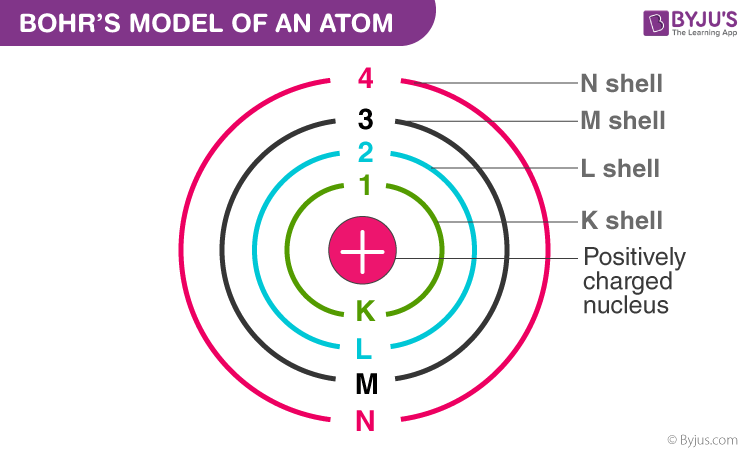
\includegraphics[width=0.75\linewidth]{atom.png}
    \caption{Structure of an atom}
\end{figure}
An atom of X element has Z number of protons, N number of neutrons [n(0)], and a mass (A) of Z+N. An element can be expressed as $\ch{^{A}_{Z}X}$ \par.
%-------------------------------------------------------------------------------------------------------------------------------------------------------------------------------------------------------------------------------------------------------------------------------------------------------------------------------------%
\section{Stability of atomic nuclei}
\begin{figure}
    \centering
    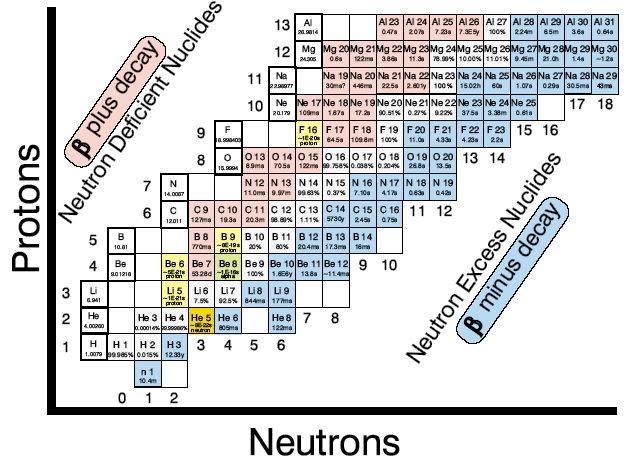
\includegraphics[width=0.75\linewidth]{chart_of_nucleides.png}
    \caption{Chart of Nucleides}
\end{figure}
%-------------------------------------------------------------------------------------------------------------------------------------------------------------------------------------------------------------------------------------------------------------------------------------------------------------------------------------%
\section{Radionucleides}
Some elements only exist as a radionucleide. Some elements exist with a very minute fraction of radioisotopes. There are also many artificial radionucleides.
%-------------------------------------------------------------------------------------------------------------------------------------------------------------------------------------------------------------------------------------------------------------------------------------------------------------------------------------%
\section{Activity and specific activity}
The nucleus of an unstable nucleide decays spontaneously to another nucleide (disintegration). Not affected by temperature, pressure, etc. Which nucleus will decay isn't predictable, but on average, it will decay. Activity is the decrease in radioactive nuclei per time.
\[A(t) := \frac{dN(t)}{dt}\]
The activity is expressed in Bq (1 disintegration per second). \\
Prefixes are used: k ($10^3$), M ($10^6$), G ($10^9$), T ($10^12$), m ($10^-3$), $\mu$ ($10^-6$), n ($10^-9$).
%-------------------------------------------------------------------------------------------------------------------------------------------------------------------------------------------------------------------------------------------------------------------------------------------------------------------------------------%
\section{Electromagnetic radiation}
Both a wave and a particle. The energy is expressed in J, or eV. $1\ eV = 1.6*10^{-19}\ J$. The binding energy of electrons on the outer shell is $\approx$ 30 eV. Photons and particles released are expressed in keV or MeV. X-rays are usually between 10 and 100 keV, while $\gamma$ radiation is usually between 100 and 1000 keV. 
%-------------------------------------------------------------------------------------------------------------------------------------------------------------------------------------------------------------------------------------------------------------------------------------------------------------------------------------%
\section{The radiation and the particles released during decay}
\subsection{$\alpha$ decay} Occurs when the nucleus is unstable, due to being too big. The parent atom $\ch{^{A}_{Z}X}$ gets split into a daughter atom $\ch{^{A-4}_{Z-2}Y}$ and an alpha particle $\ch{^{4}_{2}a}$.\\\\
\subsection{$\beta^{-}$ decay} Occurs when the nucleus is unstable, due to having an excess of neutrons. The parent atom $\ch{^{A}_{Z}X}$ gets split into a daughter atom $\ch{^{A}_{Z+1}Y}$, a beta particle $\ch{^{0}_{-1}e^{-}}$, and an anti-neutrino $\overline{v}_e$.\\\\
\subsection{$\beta^{+}$ decay} Occurs when the nucleus is unstable, due to having an excess of protons. The parent atom $\ch{^{A}_{Z}X}$ gets split into a daughter atom $\ch{^{A}_{Z+1}Y}$, a positron $\ch{^{0}_{+1}e^{+}}$, and a neutrino $v$. After a number of interactions, the positron $\beta{+}$ unites with an electron and converts its entire mass to energy. This annihilation produces 511 keV.\\\\
\subsection{Electron capture} The nucleus absorbs an electron from the electron cloud (usually from shell K -innermost). The parent atom $\ch{^{A}_{Z}X}$ absorbs an electron $\ch{^{0}_{-1}e^{-}}$, and gets split into a daughter atom $\ch{^{A}_{Z-1}Y}$, and a neutrino $v$.\\\\
\subsection{Gamma decay ($\gamma$)} Occurs when the atom is excited. The parent atom $\ch{^{A}_{Z}X*}$ gets excited and produces a daughter particle $\ch{^{A}_{Z}X}$ and a gamma ray $\gamma^{1}$. Internal conversion may occur (direct transfer of the energy of the nucleus to an electron).
\subsection{Internal conversion (IC)} Instead of $\gamma$ decay, internal conversion can occur. This is the the direct transfer of energy of the nucleus to an electron. The electron (conversion electron) is ejected from orbit with large energy, and can be detected as a $\beta^{-}$ particle, but with a sharply defined energy (unlike $\beta^{-}$, who share with neutrinos). Otherwise, can be considered a $\beta^{-}$ particle. This leaves a gap in the electron cloud, becoming unstable
\subsection{Follow-up processes: characteristic X-rays and Auger electrons} After the nucleus transfers energy to an electron or captures an electron, a vacancy is formed, filled by an electron a shell further away from the nucleus. The difference in binding energy causes the emission of characteristic X-ray spectrum (there's one emission per electron that descends = as many as electron shells there are). Due to this, other electrons may be ejected, known as Auger electrons.
%-------------------------------------------------------------------------------------------------------------------------------------------------------------------------------------------------------------------------------------------------------------------------------------------------------------------------------------%
\section{Parent-daughter relations}
After decay, the daughter nucleide may also be unstable. If the half-life is shorter, it's called ''ingrowth of activity'' (total activity grows). This must be taken into account.
%-------------------------------------------------------------------------------------------------------------------------------------------------------------------------------------------------------------------------------------------------------------------------------------------------------------------------------------%
\section{The time sequence in the decay processes}
An instable nucleide may have more than one decay process. Decay schemes explain graphically the decay. Parent level (top level), daughter level (bottom level), disintegration energy between them (Q). Increase in Z-value = right arrow; decrease in Z-value or EC = left arrow. 

\chapter{Definitions and overview of applications}%-------------------------------------------------------------------------------------------------------------------------------------------------------------------------------------------------------------------------------------------------------------------------------------------------------------------------------------%
\section{Definitions}
\textbf{Radiation sources}: entities that may cause exposure, including radioactive, X-ray, and accelerators. Some States call them \textbf{Sources}.\\\\
\textbf{Radioactive substances}: any substance that contains one or more radionuclide in the activity or activity concentration of which cannot be disregarded from a safety point of view.\\\\
\textbf{Radioactive sources}: radiation source incorporating radioactive material for the purpose of utilising its radioactivity. Include sealed and dispersible sources.\\\\
\textbf{Sealed sources}: the radioactive material is PERMANENTLY sealed in a capsule or incorporated in a solid form to prevent under normal use the dispersion of radiation.\\\\
\textbf{HASS/HAS-bron}: High Activity Sealed Source/Bron. Have additional regulations. \\\\
\textbf{Open/dispersible/unsealed sources}. there's a chance of dispersion.\\\\
\textbf{X-ray equipment}: equipment that can emit ionising radiation but doesn't contain any radioactive source, fissile material, or ore. When the equipment is off, no radiation is produced.\\\\
\textbf{Fissile material}: substances containing some percentage of uranium, plutonium, thorium, or other designated elements.\\\\
\textbf{Ore}: contain at least 10\% uranium or 3\% thorium, used for their fission or fertile properties. They are more regulated. Some substances, such as uranyl acetate (electron microscope stain) is considered a fissile material. Other States may use other definitions
\\\\\textbf{Sources of natural radiation}: may originate in the Earth or Space. Also known as NORM (Naturally Occurring Radioactive Material). Fewer regulations apply, unless used for their radioactive properties.
\\\\\textbf{Artificial sources}: sources with man-made radioactive substances.
%-------------------------------------------------------------------------------------------------------------------------------------------------------------------------------------------------------------------------------------------------------------------------------------------------------------------------------------%
\section{Overview of applications}
About 7500 licenses are granted in the Netherlands.\\ 
Academic hospitals (8 licenses) have the most extensive licenses, concerning X-ray equipment, some sealed sources, and most of the open sources in the Netherlands. \\
HASS are used in 4 companies that carry out non-destructive testing. \\
Less strong sealed sources are used in measurement and control technology. \\
Open sources are mostly used in radionuclide laboratories of universities or research institutions. \\
X-ray equipment is used in over 250 academic and non-academic hospitals and outpatient clinics, 4700 dental practices and 2400 veterinary practices. 
%-------------------------------------------------------------------------------------------------------------------------------------------------------------------------------------------------------------------------------------------------------------------------------------------------------------------------------------%
\chapter{Interaction of radiation with matter and shielding of radiation}\section{Interaction of $\beta$ radiation}
$\beta$ radiation has a spectrum between 0 and $E_{\beta,max}$. $\beta$ particles have an energy between 0 and $E_{\beta,max}$. They can be absorbed by 4 types of interactions.
\subsection{Elastic collisions}
It can collide with an electron that is strongly bound to the nucleus, without ejecting it from the orbit. The $\beta$ particle will bounce, without any energy transfer or loss, but a change in direction. This causes the particle to follow a winding path.
\subsection{Inelastic collisions}
In an inelastic collision, an electron is shot away from the electron shell, creating an ion. A $\beta$ particle has about 500x fewer ionisations per volume. Therefore, the energy is lower, but the range is higher.
\subsection{Bremsstrahlung}
When a moving electrically charged particle enters an EM field, its trajectory is deflected. This causes some energy loss, braking radiation. The higher energy of the particle and the stronger the field (Z-number), the higher this effect is. It is approximately:
\[g \approx 2\cdot10^4\cdot Z\cdot E_{\beta,max}\]
Perspex blocks well, and causes low Bremsstrahlung.
\subsection{Čerenkov radiation}
For a $\beta$ particle with energy >250keV, the speed approaches the speed of light. In water, a high energy particle may travel faster than light, emitting energy in the form of photons in the blue to violet region. The light may be visible to the naked eye. This does not slow the particles much.
\subsection{Annihilation ($\beta^+$)}
Occurs when a $\beta^+$ particle collides with an electron at the end of its path. They both get converted to 2 photons of 511keV each.
%-------------------------------------------------------------------------------------------------------------------------------------------------------------------------------------------------------------------------------------------------------------------------------------------------------------------------------------%
\section{Interaction processes of X-rays and $\gamma$ radiation}
See section 3.5 of book.
%-------------------------------------------------------------------------------------------------------------------------------------------------------------------------------------------------------------------------------------------------------------------------------------------------------------------------------------%
\section{Shielding of $\beta$ radiation}
The range of $\beta$ radiation can be calculated with
\[R_{\beta,\ in\ material} = \frac{R_{\beta,\ in\ water} = 0.5 E_{\beta,max}}{\rho_{material}}\]
For water and tissue, $\rho$ can be estimated to be 1 g/cm³. $E_{\beta,max}$ is expressed in MeV.\\
%-------------------------------------------------------------------------------------------------------------------------------------------------------------------------------------------------------------------------------------------------------------------------------------------------------------------------------------%
\section{Shielding of a narrow beam of X-rays and of $\gamma$ radiation}
We are ignoring scattering/buildup.
\[I(d) = I(0)\cdot B\cdot(\frac{1}{2})^{\frac{d}{d_{1/2}}}\]
Buildup factor (P60) may often be ignored. All distance units must be in the same unit. The buildup factor increases with increasing half-thicknesses. With lead, it won't exceed 5 if <14 half-thicknesses are applied. For ther materials, it can reach >20.\\
\[I(d) = I(0)\cdot e^{-\mu_{linear} d}; \mu_{mass} = \mu_{linear}\cdot\rho_{material}^{-1}\]
Above 500keV, $\mu_{mass\ water}\approx\mu_{mass\ concrete}$.\\

\chapter{Quantities and units in radiation protection}\section{Quantities and units describing the risk}
\subsection{Absorbed dose}
The absorbed dose (D) is the energy absorbed per unit mass. The unit is the Gray (Gy), which equals 1 J/kg. 1 Gy \approx 100 Röntgen. The absorbed dose rate is Gy/h.

\subsection{Equivalent dose}
The equivalent dose depends on the type of radiation. 
\[H_T=W_R\cdot D\]
Where $H_T$ is the absorbed dose for tissue and organ, $W_R$ is the radiation weighting factor (1 for $\beta$ and $\gamma$, 20 for $\alpha$ particles, and 2-20 for neutrons. Its unit is the same as for absorbed dose, but is called Sievert (Sv).

\subsection{Effective dose}
An equivalent dose for the whole body correlates with a higher risk than an equivalent dose in a part of the body. This is what the Effective Dose is for. It gives an approximation of the total body dose. The equivalent dose for each tissue is multiplied by a $W_T$ tissue weighting factor.
\[E=\sum W_T \cdot H_T = \sum W_T \cdot W_R \cdot D\]

\subsection{Committed dose}
After an intake of radioactive substances in the body, tissues will be irradiated. The equivalent dose caused by this is calculated with the committed equivalent dose $H_T(50)$ (50 = summation period of 50 years for adults).
\[E(50) = e(50)\cdot A\]
Where e(50) is the committed dose coefficient. These coefficients vary, and depend on the rate of excretion, physical decay, and uptake paths. Some substances can enter the body in different ways, so there's different e(50) for inhalation, ingestion and inoculation.
%-------------------------------------------------------------------------------------------------------------------------------------------------------------------------------------------------------------------------------------------------------------------------------------------------------------------------------------%
\section{Quantities and units in measurements}
Measurements are often not fully accurate, and approximations are taken. 
\subsection{H*(10) and H*(0.07)}
A phantom is an object that mimics the human body, in this case, a sphere of diameter 30cm. A measurement of the equivalent dose is done at a depth of 10 mm in the phantom, which is a good estimate of the effective dose of a human standing in a parallel incident radiation field. The H*(10) is based on this, and it's called the ambient dose equivalent (Sv). Below 100 keV, this causes an overestimation of E. For photons under 50 keV, this can lead to up to 5x overestimation. It's only a good measure for whole-body irradiation. If only part of the body is irradiated, it is a good measure for the equivalent dose to that part of the body. However, it's only aq good measure if the body is irradiated from front to back. If the irradiation is back to front, it causes a 30\% overestimation. It is not a good equivalent for the skin dose, for which H*(0.07) is used.
\chapter{Radiation detection}\section{Detector material}
Depending on the material of the detector, different types of radiation can be measured.
%-------------------------------------------------------------------------------------------------------------------------------------------------------------------------------------------------------------------------------------------------------------------------------------------------------------------------------------%
\section{Ionisation detectors}
\subsection{Gas-filled}
\subsubsection{The ionisation chamber}
In the ionisation chamber, the applied voltage between cathode and anode is low, but large enough to prevent recombination of the electron-ion pair. If they recombine into a neutral molecule, no current pulse will be formed. If electron-ion pairs, they can be detected as an electric pulse. It's rarely used, as it is tricky to process the data. It may be used when the dose rate is very high.
\subsubsection{The proportional counter}
Using a higher voltage causes a stronger electric field, in which the electrons are accelerated to such high energies that they cause new ionizations. As a consequence, the signal will be increased proportionally. The thin window allows for detection of $\alpha$ and $\beta$ particles. To boost X-ray and low-energy $\gamma$ radiation, a high-Z-value gas is used.
\subsubsection{GM tube}
The GM tube uses a higher voltage, and regardless of the energy, each incident particle will cause an avalanche of electron-ion pairs. It's useful for small-surface contaminations. It's mostly a qualitative (boolean) measurement.
\subsection{Solid-state semiconductor detectors}
These are very expensive to use, as they require tons of active cooling. However, they give a very detailed spectrum of energies released.
%-------------------------------------------------------------------------------------------------------------------------------------------------------------------------------------------------------------------------------------------------------------------------------------------------------------------------------------%
\section{Scintillation detectors}
\subsection{Solid state scintillation detectors}
Most notable is ThermoLuminescence Detectors (TLDs), used in personal dosimeter badges. The radiation is "stored" as electrons, and can be released with heat.
\subsection{Liquid scintillation}
Liquid scintillation is an organic solvent with an organic scintillator. The sample being dissolved in here helps it detect even extremely low energy samples.
%-------------------------------------------------------------------------------------------------------------------------------------------------------------------------------------------------------------------------------------------------------------------------------------------------------------------------------------%
\section{Application of radiation detection in radiation protection}
\subsection{Identification of a source}
Sometimes, the nuclide is unknown. When there's a limited number of possibilities, different shielding materials can be used to compare activity after half-thicknesses with theoretical values. The energy can be measured, or solid state detectors can be used to get a spectrum.
\subsection{Determination of the activity}
Activity can be estimated by holding the source in front of a contamination monitor. For more precise applications, various detectors can be used.
\subsection{Determination of the dose rate}
Dose rate from $\beta$ and $\gamma$ particles can be measured with a dosimeter. 
\subsection{Measurement of active contamination}
Contamination monitors are used to determine whether radioactivity is present. These contamination monitors are much more sensitive than dosimeters. For small areas, simple GM tubes are used for $\beta$, while NaI crystals are used for $\gamma$. For $\alpha$, ZnS scintillation detectors are used, though a swipe test and liquid scintillation count is more effective. \\
Proportional counters can be used for large surface contaminations. A Hand Feet Clothes monitor is used at the exit of the laboratory, to check whether there is contamination.
%-------------------------------------------------------------------------------------------------------------------------------------------------------------------------------------------------------------------------------------------------------------------------------------------------------------------------------------%
\chapter{Biological effects and risks of radiation}\section{Introduction}
%-------------------------------------------------------------------------------------------------------------------------------------------------------------------------------------------------------------------------------------------------------------------------------------------------------------------------------------%
\section{Effects at the molecular and cellular level}
%-------------------------------------------------------------------------------------------------------------------------------------------------------------------------------------------------------------------------------------------------------------------------------------------------------------------------------------%
\section{Effects in humans}
%-------------------------------------------------------------------------------------------------------------------------------------------------------------------------------------------------------------------------------------------------------------------------------------------------------------------------------------%
\section{Harmful tissue reactions}
%-------------------------------------------------------------------------------------------------------------------------------------------------------------------------------------------------------------------------------------------------------------------------------------------------------------------------------------%
\section{Stochastic effects}
%-------------------------------------------------------------------------------------------------------------------------------------------------------------------------------------------------------------------------------------------------------------------------------------------------------------------------------------%
\section{Effects on offspring}
%-------------------------------------------------------------------------------------------------------------------------------------------------------------------------------------------------------------------------------------------------------------------------------------------------------------------------------------%
\section{Effects on the unborn child}
%-------------------------------------------------------------------------------------------------------------------------------------------------------------------------------------------------------------------------------------------------------------------------------------------------------------------------------------%
\section{Comparison with other risks}
\chapter{Regulations and ethics}\section{Terminology}
\textbf{Exposed worker/Radiation worker} Employee exposed to >1mSv/y. \\\\
\textbf{Practices} Everything that may increase one's exposure. Including storage.\\\\
\textbf{RPO/TMS} Technically competent in a specific branch of radiation protection. 9 groups: medical applications, dentistry, veterinary X-ray, nuclear fuel cycle, dispersible radiation substances, NORM, accelerators, industrial radiography, mesurement and control applications. See Annex 5.2 of Rbs for training requirements. Every company that works with ionising radiation must employ an RPO, RPO does not have to be recorded in a national register.\\\\
\textbf{RPE} Gives advice about radiation protection and is recognised by the State as an expert. They also have supervisory tasks.\\\\
\textbf{Radiation expert} RPOs and RPEs \\\\
\textbf{Undertaking} The person (or company) under whose responsibility a practice is carried out or a measure is taken.\\\\
\textbf{Exposure situations} Planned exposure situations, radiological emergency situations (immediate action), existing exposure situations.\\\\
\textbf{Radiation incident} An unintended event or situation or unintended spread of activity, in which there is or is danger of exposure to ionising radiation by public of >0.1 mSv, discharge to or into the soil, sewer, surface water or air above a specific level, or an exposure to ionising radiation of workers exceeding 2 mSv. This must be reported.\\\\
\textbf{Anticipated and non-anticipated unintended event} Whether it's in the radiation risk inventory and evaluation \\\\
\textbf{Reporting obligations} Radiation incidents + non-anticipated unintended events + anticipated unintended events if dose is higher than predicted.\\\\
%-------------------------------------------------------------------------------------------------------------------------------------------------------------------------------------------------------------------------------------------------------------------------------------------------------------------------------------%
\section{The system of radiation protection}
\textbf{Justification} The application must be justified, and no alternative non-ionising methods must exist. Pros and cons must be evaluated as individual and society (present and future). Annex 2.1 of Rbs includes justified examples. RPO and radiation worker won't notice justification, as license has also been granted.\\\\
\textbf{ALARA/optimisation}  As Low As Reasonably Achievable. Even if the dose is already low, it should be lowered if possible. It concerns everyone, present and future. Dose constraints contain ALARA (not LIMITS, these are guidances). An undertaking must establish dose constraints below the limits, unless practice results in extremely low exposure. Dose constraing of 10 $\mu$Sv as an annual dose for the public, 100x lower than the limit. ALARA is applied as a source-oriented strategy: examine whether a less risky source is possible, containing the source, shielding the source, increasing the distance between the source and the individual, and as a last step, personal measures. Reasonable = 1€ to save 10 $\mu$Sv (QALY). \\\\
\textbf{Dose limitation}  The limits are there to avoid too high a dose for an individual. They should not be used as a guide for a maximum permissible dose, they CANNOT be exceeded, and act as a safety net. See table in QRH for dose limits. The annual limit for Cat. A is almost never exceeded in the Netherlands. Dose limits do not apply to patients, or to an existing exposure situation, or to a radiological emergency, which are then reference levels. For existing exposure situations the limit is between 1 and 20 mSv/y. For emergencies, it is between 20 and 500 mSv, depending on the severity, the possibilities for taking protecive measures, and the role in the emergency response. In an emergency, anything over 100 mSv requires informed consent.\\\\
%-------------------------------------------------------------------------------------------------------------------------------------------------------------------------------------------------------------------------------------------------------------------------------------------------------------------------------------%
\section{Regulations at the workplace}
Before a new practice is carried out, a risk inventory and evaluation (Risk Assessment) must be carried out. Radiation risks during normal operations are considered, but also anticipated unintended effects (fire, loss of source, etc). The RPO will draft a concept, and the RPE will ratify it. The RA must be adapted when there's new developments, and at most must be revised every 5 years. Instruction must be given, including of all local protocols, as well as emergency protocols. Women need extra information. \\
Category A workers must receive a yearly medical visit by a registered medical radiation specialist, also before and after the employment, as well as yearly thereafter. \\
Category A and Category B workers must have a TLD badge or personal dosimeter. Category C \textbf{MUST? NOT HAVE IT}. \\
A controlled area is where it's possible to get > 6mSv/y effective dose. A supervised area it's between 1 adn 6 mSv/y effective dose. If a dose rate of > 10 $\mu$Sv/h can occur, a special sign must be placed stating so. Class B laboratory and workplace with an accelerator are controlled. Classs C and workplace with X-ray devices is supervised. Category B workers can work in controlled areas in specific circumstances. \\
The storage facility must be fire resistant for >60 mins. The dose rate outside must be <1 $\mu$Sv/h. The storage facility must be easy to decontaminate and a ventilation rate of 3x/h if dispersible sources are used.\\
TLD badges for Class A and B employees have their data recorded in NDRIS (National Dose Registration and Information System). This data must be kept until the age of 75 of the employee, OR AT LEAST 30 years after the termination of the work, whichever is longer. The badge is worn on the collar, mid-torso or waist with the label facing out; on top of an apron if it's worn. If the worker always wears an apron, the TLD company must take this into account, and a correction factor of 0.2 will apply only if the lead aprons are adequate, in the medical profession, and the voltage of X-ray apparatus is <125 kV. \\
Any information relevant for radiation protection must be kept in the Nuclear Energy Act File.
%-------------------------------------------------------------------------------------------------------------------------------------------------------------------------------------------------------------------------------------------------------------------------------------------------------------------------------------%
\section{Regulations regarding security}
The security category of a source is determined by the A (activity)/D-value. For an A/D <1, no special security measures are needed, but it's necessary to prevent loss, robbery, or dispersion. 
%-------------------------------------------------------------------------------------------------------------------------------------------------------------------------------------------------------------------------------------------------------------------------------------------------------------------------------------%
\section{Transport regulations}
Any transport should be done by an ADR-certified carrier. The transport must be notified 3 weeks in advance to the ANVS; unless done by an ADR, in which case it's a yearly notification and no 3-week notice is needed; unless for fissile material, where a license is needed. \\\\
Packages (collo/colli). For an exempted package, the total activity and activity concentration are so low, no labelling is needed. The TI level must be specified, it's 0.1x ($\mu$Sv) the radiation level 1m away from the collo. A safety label is needed:\\
\begin{enumerate}
\item I - White. Radiation level on collo surface <5 $\mu$Sv/h.
\item II - Yellow. Radiation level on collo surface <500 $\mu$Sv/h, >5 $\mu$Sv/h, must not exceed 10 $\mu$Sv/h at 1m.
\item III - Yellow. Radiation level on collo surface <2000 $\mu$Sv/h (limit MAY be exceeded in some conditions), >500 $\mu$Sv/h, must not exceed 100 $\mu$Sv/h at 1m, but higher than 10 $\mu$Sv/h at 1m.
\end{enumerate}

\chapter{Dosimetry in practice}\section{External irradiation by a radioactive source emitting $\gamma$ radiation}
The 10 H(10) refers to the depth in mm in a phantom (tissue equivalent)
\subsection{Time}
The duration of the exposure determines the ambient dose equivalent:
\[H^*(10)=\dot{H}^*(10)\cdot t\]
\subsection{Distance}
Radiation follows the inverse square law
\[\dot{H}^*(10)(10) = h(10)\cdot\frac{A}{r^2}\]
\subsection{Shielding}
For $\gamma$ radiation, it applies that
\[I(d) = I(0)\cdot B\cdot(\frac{1}{2})^{\frac{d}{d_{1/2}}}\]
Therefore
\[\overset{.}{H^*}(10)_{shielding} = \dot{H}^*(10)(10)_{raw} \cdot B\cdot(\frac{1}{2})^{\frac{d}{d_{1/2}}}\]
\subsection{Full formula for the ambient dose equivalent rate}
\begin{equation}
    \dot{H}^*(10)_{\text{(at distance r, with shielding d)}} = h(10) \cdot \frac{A}{r^2} \cdot B \cdot \left(\frac{1}{2}\right)^{\frac{d}{d_{1/2}}}
    \label{eq:placeholder}
\end{equation}
\subsection{Rule of thumb for $\gamma$ radiation}
\[\dot{H}^*(10) = 2A \approx \dot{E}\]
With A in MBq and $\dot{H}^*(10)$ in $\mu$Sv/h. For $\dot{E}$, this is at a distance of 30cm from the source, without shielding.
%-------------------------------------------------------------------------------------------------------------------------------------------------------------------------------------------------------------------------------------------------------------------------------------------------------------------------------------%
\section{Skin irradiation}
\subsection{Rule of thumb for external radiation of the skin by $\beta$ (+ and -) radiation}
\[\dot{H}^*(0.07) = 1000\cdot A\]
This formula is for a source 10 cm away from the skin without shielding. \\
Where the 0.07 represents a depth of 0.07 mm in a phantom, representing the top layer of skin. The annihilation photons ($\beta^+$) have a negligible contribution.

\subsection{Rule of thumb for external contamination of the skin by $\beta$ (+ and -) radiation}
\[\dot{H}^*(0.07) = 2000\cdot A\]
With A units of kBq/cm².

%\chapter{[OPTIONAL] Industrial radiography and measurement and control applications}\section{Introduction}
%-------------------------------------------------------------------------------------------------------------------------------------------------------------------------------------------------------------------------------------------------------------------------------------------------------------------------------------%
\section{Definitions}
%-------------------------------------------------------------------------------------------------------------------------------------------------------------------------------------------------------------------------------------------------------------------------------------------------------------------------------------%
\section{Sealed sources}
%-------------------------------------------------------------------------------------------------------------------------------------------------------------------------------------------------------------------------------------------------------------------------------------------------------------------------------------%
\section{X-rays}
%-------------------------------------------------------------------------------------------------------------------------------------------------------------------------------------------------------------------------------------------------------------------------------------------------------------------------------------%
\section{Regulations for IR and MCA}
%-------------------------------------------------------------------------------------------------------------------------------------------------------------------------------------------------------------------------------------------------------------------------------------------------------------------------------------%
\section{Workplace measures for IR applications}
%-------------------------------------------------------------------------------------------------------------------------------------------------------------------------------------------------------------------------------------------------------------------------------------------------------------------------------------%
\section{Workplace measures for MCA}
\chapter{Safety measures for open sources}\section{Introduction}
%-------------------------------------------------------------------------------------------------------------------------------------------------------------------------------------------------------------------------------------------------------------------------------------------------------------------------------------%
\section{Elaboration on the legal framework}
%-------------------------------------------------------------------------------------------------------------------------------------------------------------------------------------------------------------------------------------------------------------------------------------------------------------------------------------%
\section{Reducing activity}
%-------------------------------------------------------------------------------------------------------------------------------------------------------------------------------------------------------------------------------------------------------------------------------------------------------------------------------------%
\section{Containment}
%-------------------------------------------------------------------------------------------------------------------------------------------------------------------------------------------------------------------------------------------------------------------------------------------------------------------------------------%
\section{Removal of airborne contamination}
%-------------------------------------------------------------------------------------------------------------------------------------------------------------------------------------------------------------------------------------------------------------------------------------------------------------------------------------%
\section{Individual protection}
%-------------------------------------------------------------------------------------------------------------------------------------------------------------------------------------------------------------------------------------------------------------------------------------------------------------------------------------%
\section{Contamination check and decontamination}%-------------------------------------------------------------------------------------------------------------------------------------------------------------------------------------------------------------------------------------------------------------------------------------------------------------------------------------%
\section{Radioactive waste}
%-------------------------------------------------------------------------------------------------------------------------------------------------------------------------------------------------------------------------------------------------------------------------------------------------------------------------------------%
\section{Topics}
\end{document}